%==================================\textit{}=============================
%Template for UPC-TALP based on CTU and modified to match UPC-TALP colors and style  
%The original template from Czech Technical University  % Author: Martin Malý.
% They are defined by new graphical manual - 2017.
% Share and modify as you like. Keep the name of the authors.
% It is forbidden to use the template commercially.
%===============================================================

\documentclass{beamer}
\usepackage[utf8]{inputenc}
%\usepackage{lmodern}
\usepackage{relsize}

\usepackage{algorithm}
\usepackage{amsthm}
\usepackage{algpseudocode}
\usepackage{comment}
\usetheme{Madrid}
  \usepackage[maxbibnames=99]{biblatex}
\definecolor{main_color}{HTML}{BD5045}
\definecolor{end_title_color}{HTML}{9D4035}
\usepackage{biblatex}
%\usepackage{tikz}
%\usepackage{pgfplots}
\usepackage[makeroom]{cancel}
\usepackage{threeparttable}
\usepackage[utf8]{inputenc}
%\usepackage[usenames,dvipsnames]{xcolor}
%\addbibresource{biblatex-examples.bib}
%\setbeamercolor{section in toc}{}
\setbeamercolor{section in toc}{fg=black,bg=yellow}
\usepackage{tikzsymbols}
\usepackage{textcomp}
\usepackage{parskip}
\usepackage{pgf}
\usepackage{color,soul}
%\usepackage{pythontex} 
\usepackage{tcolorbox}
\tcbuselibrary{skins}
\usepackage{minted}
\usepackage{hyperref}
\usepackage{amsmath}
\usepackage{amssymb}
\usepackage{xcolor,soul}
\renewcommand<>{\hl}[1]{\only#2{\beameroriginal{\hl}}{#1}}
\setbeamertemplate{page number in head/foot}[framenumber]
%%% attravive box over equestion
\usepackage{empheq}
\usepackage{xcolor}
\definecolor{lightgreen}{HTML}{90EE30}
\newcommand{\boxedeq}[2]{\begin{empheq}[box={\fboxsep=6pt\fbox}]{align}\label{#1}#2\end{empheq}}
\newcommand{\coloredeq}[2]{\begin{empheq}[box=\colorbox{lightgreen}]{align}\label{#1}#2\end{empheq}}
\newcommand{\highlight}[1]{%
\colorbox{red!40}{$\displaystyle#1$}}
  
  
\definecolor{babyblue}{rgb}{0.94, 0.54, 0.31}
\newcommand{\bert}{\ensuremath{%
  \mathchoice{\includegraphics[height=2ex]{Bert-pic-removebg-preview.png}} 
    {\includegraphics[height=2ex]{Bert-pic-removebg-preview.png}}
    {\includegraphics[height=1.5ex]{Bert-pic-removebg-preview.png}}
    {\includegraphics[height=1ex]{Bert-pic-removebg-preview.png}}
}}
  
  
\useoutertheme{infolines}



\usepackage{courier}
%\usepackage{animate}  
\usepackage{expl3}
%\usepackage[listings,theorems]{tcolorbox}



%%%%%%%%%%%%%%%%%%%%%%%%%%%%%%%%%%%%%%%%%%%%%%%%%%%%%%%%%%%%%%%%%%%%%  
%commands for simulating terminal in/output  
%\scroll[<line separator string>]{<width as TeX dim>} 
%                             {<number of lines>}{terminal text line}  
%\clearbuf  %clears line buffer  
%%%%%%%%%%%%%%%%%%%%%%%%%%%%%%%%%%%%%%%%%%%%%%%%%%%%%%%%%%%%%%%%%%%%%  



\newcommand\scroll[4][§§]{
  \seq_set_split:Nnn\g_inputline_seq{#1}{#4}
  \seq_map_inline:Nn\g_inputline_seq{
    \seq_gput_right:Nx\g_linebuffer_seq{##1}
    \int_compare:nT{\seq_count:N\g_linebuffer_seq>#3}{
      \seq_gpop_left:NN\g_linebuffer_seq\dummy
    }
  }
  \fbox{\begin{minipage}[t][#3\baselineskip]{#2}
    \ttfamily
    \seq_map_inline:Nn\g_linebuffer_seq{\mbox{##1}\\}
  \end{minipage}}
}
\newcommand\clearbuf{\seq_gclear:N\g_linebuffer_seq}
\ExplSyntaxOff

\setbeamertemplate{headline}{%
\begin{beamercolorbox}[colsep=1.5pt]{upper separation line head}
\end{beamercolorbox}
\begin{beamercolorbox}{section in head/foot}
    \vskip2pt\insertsectionnavigationhorizontal{\paperwidth}{}{\hskip0pt plus1fill}\vskip2pt
\end{beamercolorbox}%

\begin{beamercolorbox}[colsep=1.5pt]{lower separation line head}
\end{beamercolorbox}
}
\makeatletter
\newcommand\SoulColor{%
  \let\set@color\beamerorig@set@color
  \let\reset@color\beamerorig@reset@color}
\makeatother
\SoulColor
\usepackage{amsmath, bm}
\usepackage{tikz}
\setbeamercovered{dynamic}

\newcommand{\highlightt}[1]{%
  \colorbox{red!40}{$\displaystyle#1$}}


\newenvironment<>{problock}[1]{%
  \begin{actionenv}#2%
      \def\insertblocktitle{#1}%
      \par%
      \mode<presentation>{%
       \setbeamercolor{block title}{fg=white,bg=end_title_color}
       \setbeamercolor{block body}{fg=black,bg=white!50}
       \setbeamercolor{itemize item}{fg=orange!20!black}
       \setbeamertemplate{itemize item}[triangle]
     }%
      \usebeamertemplate{block begin}
    \par\usebeamertemplate{block end}
    \end{actionenv}
    }
    
    \newcommand<>{\uncovergraphics}[2][{}]{
    % Taken from: <https://tex.stackexchange.com/a/354033/95423>
    \begin{tikzpicture}
    \node[anchor=south west,inner sep=0] (B) at (4,0)
        {\includegraphics[#1]{#2}};
    \alt#3{}{%
        \fill [draw=none, fill=background, fill opacity=0.9] (B.north west) -- (B.north east) -- (B.south east) -- (B.south west) -- (B.north west) -- cycle;
    }
    \end{tikzpicture}
}




\newlength\dlf
\newcommand\alignedbox[3][yellow]{
  % #1 = color (optional, defaults to yellow)
  % #2 = before alignment
  % #3 = after alignment
  &
  \begingroup
  \settowidth\dlf{$\displaystyle #2$}
  \addtolength\dlf{\fboxsep+\fboxrule}
  \hspace{-\dlf}
  \fcolorbox{red}{#1}{$\displaystyle #2 #3$}
  \endgroup
}

\usepackage{collcell}
\usepackage{booktabs}
\usepackage{etoolbox}
%\usepackage{remreset}% tiny package containing just the \@removefromreset command
\makeatletter

\usepackage{xcoffins}
\NewCoffin\tablecoffin
\NewDocumentCommand\Vcentre{m}
  {%
    \SetHorizontalCoffin\tablecoffin{#1}%
    \TypesetCoffin\tablecoffin[l,vc]%
  }



\usepackage{pgfpages}

%% Important 
%%% show note or disable note. 
%\setbeameroption{show notes on second screen=right} % Both

\setbeamertemplate{note page}{\pagecolor{gray!5}\insertnote}\usepackage{palatino}

\usepackage{xcolor}
\usepackage{soul}

\usepackage{etoolbox}
\makeatletter
%\patchcmd{\slideentry}{\ifnum#2>0}{\ifnum2>0}{}{\@error{unable to patch}}% replace the subsection number test with a test that always returns true
\makeatother

\setbeamercolor*{palette primary}{bg=main_color,fg=gray!20!white}
\setbeamercolor*{palette secondary}{bg=main_color,fg=gray!20!white} % no color
\setbeamercolor*{palette tertiary}{parent=palette primary} % color of the top and date
\setbeamercolor*{palette quaternary}{fg=main_color,bg=gray!5!white}
\setbeamercolor*{sidebar}{fg=main_color,bg=gray!15!white}
\usepackage[first=0,last=9]{lcg}
\newcommand{\ra}{\rand0.\arabic{rand}}
\usepackage{color, colortbl}
\usepackage{stackengine,tikz}
\usepackage{transparent}
\usepackage{pgfpages}

\usepackage{booktabs}% http://ctan.org/pkg/booktabs

\colorlet{Gray}{gray!30}

\usepackage{mathtools}

\DeclarePairedDelimiterX{\infdivx}[2]{}{}{%
  #1\;\delimsize\|\;#2%
}
\newcommand{\infdiv}{D\infdivx}
\DeclarePairedDelimiter{\norm}{\lVert}{\rVert}





    
\newcommand*{\MinNumber}{0}%
%\newcommand*{\MaxNumber}{100}%
\newcommand*{\MaxNumber}{0.4}%
\definecolor{bubblegum}{rgb}{0.99, 0.76, 0.8}
\newcommand{\ApplyGradient}[1]{%
  \pgfmathsetmacro{\PercentColor}{100.0*(#1-\MinNumber)/(\MaxNumber-\MinNumber)}%
  %\textcolor{black!\PercentColor}{#1}
  \edef\x{\noexpand\cellcolor{babyblue!\PercentColor}}\x\textcolor{black}{#1}%
}
\newcolumntype{R}{>{\collectcell\ApplyGradient}{c}<{\endcollectcell}}

%\setbeameroption{show notes on second screen=right}
\setbeamercolor{titlelike}{parent=palette primary}
\setbeamercolor{frametitle}{parent=palette primary}

\setbeamercolor{B}{bg=red!30,fg=black}


\setbeamertemplate{section in toc}[default]
\setbeamercolor{itemize item }{fg=red}
\setbeamertemplate{itemize item}[circle]

\setbeamercolor*{separation line}{}
\setbeamercolor*{fine separation line}{}

\setbeamertemplate{navigation symbols}{} 
\setbeamertemplate{caption}{\raggedright\insertcaption\par}


\setbeamercolor*{block title example}{fg=white,bg=purple!75!black}
\setbeamercolor*{block body example}{fg= black, bg= white}


\setbeamercolor{itemize item}{fg=main_color} % all frames will have red bullets
\setbeamercolor{block title}{bg=red!30,fg=black}
\setbeamertemplate{subsection in toc}[subsections numbered]


\usepackage{eqnarray,amsmath}
\usepackage{amsfonts}
\usepackage{amssymb}
\usefonttheme{professionalfonts}
\usepackage{graphicx}
\usepackage{booktabs} 
\usepackage{bm}
\usepackage{mathtools}
\usepackage[utf8]{inputenc}
\usepackage[T1]{fontenc}
\usepackage{lmodern} 
\usepackage{booktabs}

\setbeamercolor{block title}{fg=black, bg=yellow}
\setbeamercolor{block2}{use=structure,fg=white,bg=purple!75!black}
% definice makra
\def\bq{\mbox{\kern.1ex\protect\raisebox{-1.3ex}[0pt][0pt]{''}\kern-.1ex}}
\def\eq{\mbox{\kern-.1ex``\kern.1ex}}
\def\ifundefined#1{\expandafter\ifx\csname#1\endcsname\relax }%
\ifundefined{uv}%
        \gdef\uv#1{\bq #1\eq}
\fi


%====================================================
%========== DEFINITION OF AUTHORS ETC...=============
%====================================================

\author[basnia, moorea7, woffos]{Anthony Basnight, Alex Moore, Scott Wofford}

\title[]{Stochastic Variational Inference}

%====================================================
%========== BEGINNING OF DOCUMENT ===================
%====================================================



\begin{document}



\begin{frame}[plain]
	\titlepage
\end{frame}



\begin{frame}[plain]{Table of Contents}
    \tableofcontents[]
\end{frame}



\section{Background}



\begin{frame}{Introduction}
    \begin{itemize}
        \item Paper: Stochastic Variational Inference
        \begin{itemize}
            \item Published: May 2013
            \item Authors: Matthew D. Hoffman, David M. Blei, Chong Wang, John Paisley
        \end{itemize}
    \end{itemize}
\end{frame}



\begin{frame}{Background}	
    \begin{itemize}
        \item How can we discover themes in text, organize by subject, and build a navigator for users to explore an archive of two million books?
        \item How can we recommend items to online shoppers using a database containing millions of users’ purchase histories?
        \item How can we build a classifier from a continuously collected data set of an online feed of photographs?
        \item How can we make hypotheses about connections between observed genes and other traits using the gene sequences of millions of people?
    \end{itemize}  
\end{frame}



\begin{frame}
    \begin{center}
        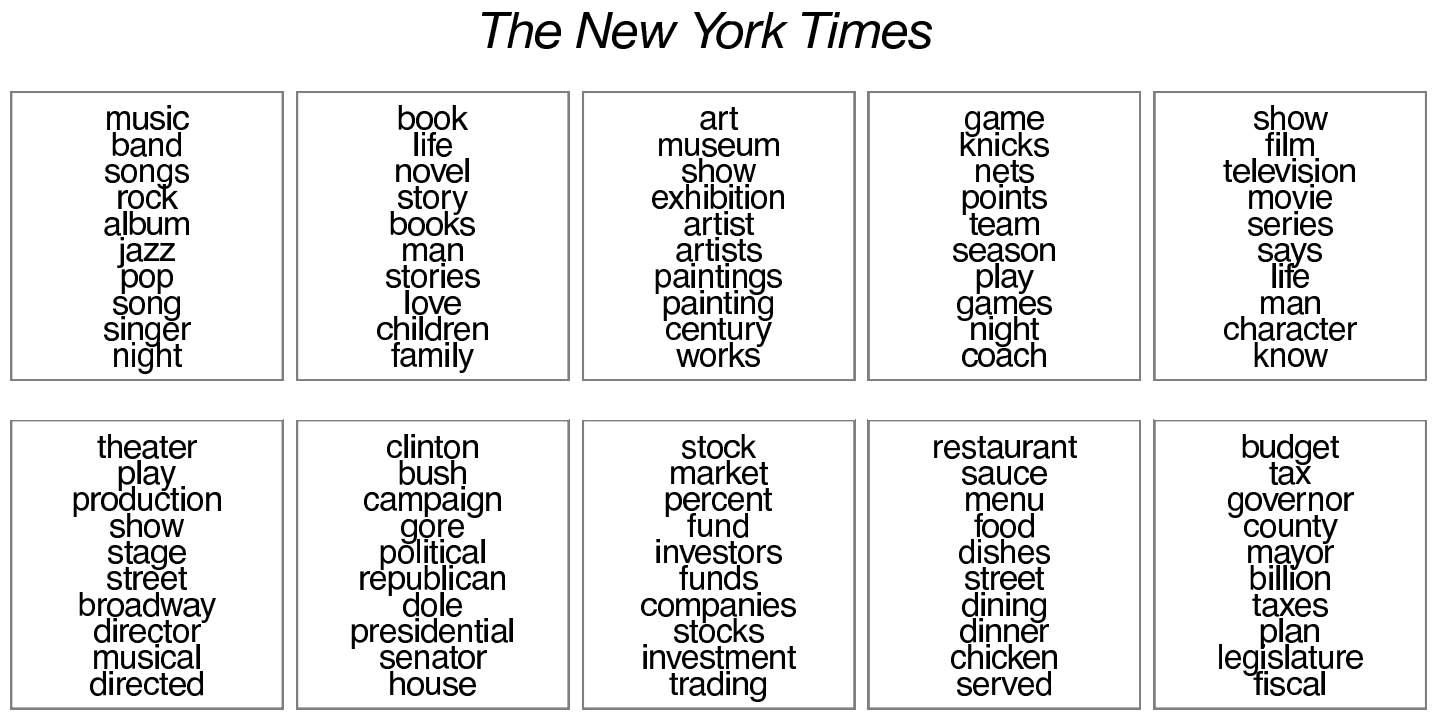
\includegraphics[width=\textwidth]{images/nyt.PNG}
    \end{center}
\end{frame}



\begin{frame}{Modeling Documents and Their Hidden Parameters}
        We view each document as a bag of words.  This means we do not care about the ordering of the words but only the number of occurrences of each word in a document.

        Each document is assigned a distribution of topics and each topic is assigned a distribution of words.  By composing these two distributions, we get the distribution of words in the document.

        Our goal is to find the find the posteriors of these distribution by sampling from many documents.
        $$p(z,\beta | x) = \frac{p(x,z,\beta)}{\int p(x,z,\beta)dzd\beta}$$
\end{frame}



\begin{frame}
    We use the following plate notation to represent documents.

    \begin{center}
        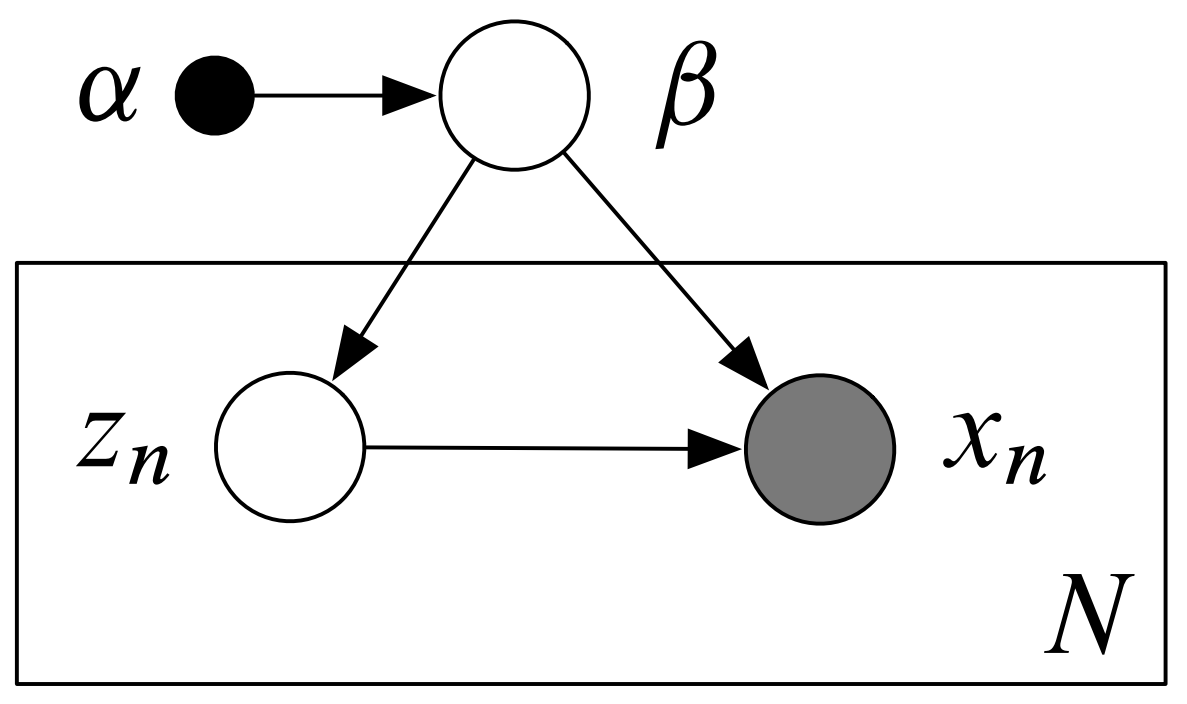
\includegraphics[width=5cm]{images/document_model.PNG}
    
    {\scriptsize
    \begin{tabular}{ |c|c|c| }
    
        \hline
            Symbol & Name & Corresponds to: \\
        \hline
            $\alpha$ & Hyper Parameters & \\
        \hline
            $\beta$ & Global Hidden Parameters &  Distribution of Words Among Topics  \\
        \hline
            $z_n$ & Local Hidden Parameters & Topic at index $n$ \\
        \hline
            $x_n$ & Observation & Word at index $n$ \\
        \hline
    \end{tabular}
    }

    \end{center}

    

\end{frame}



\begin{frame}{Topic Modeling}
    \begin{itemize}
        \item In natural language processing, topics can be thought of as “soft clusters” of words that are frequently found near each other or in the same document. They are useful for finding connections between words and finding underlying themes in documents.
        \begin{itemize}
            \item It is useful to think of the probability of a word as being conditional on the topic \\
            \bigskip
            {\scriptsize
            \begin{tabular}{ |c|c|c|c|c|c| }
                \hline
                & Word 1 & Word 2 & $\dots$ & Word V-1 & Word V \\
                \hline
                Topic 1 & 0.07 & 0.11 & $\dots$ & 0.22 & 0.05 \\
                \hline
                Topic 2 & 0.22 & 0.12 & $\dots$ & 0.19 & 0.17 \\
                \hline
                $\vdots$ & $\vdots$ & $\vdots$ & $\ddots$ & $\vdots$ & $\vdots$ \\
                \hline
                Topic K & 0.04 & 0.18 & $\dots$ & 0.08 & 0.11 \\
                \hline
            \end{tabular}
            }
        \end{itemize}
    \end{itemize}
\end{frame}



\section{Variational Inference}



\begin{frame}{Finding the Underlying Distributions}
    \begin{itemize}
        \item Main goal: Find underlying distributions
            \begin{itemize}
                \item Distribution of topics within documents: ${\bf \theta}$
                \item Distribution of words within topics: ${\bf \beta}$
            \end{itemize}
        \item Fit statistical models to approximate the distributions
        \begin{itemize}
            \item Statistical models include: Latent Dirichlet Allocation and Hierarchical Dirichlet Process
            \item Optimization methods include: Variation Inference, Mean-Field Variational Inference, Stochastic Variational Inference
        \end{itemize}
    \end{itemize} 
\end{frame}



\begin{frame}{Variational Inference (VI)}
    \begin{itemize}
        \item The joint distribution consists of a global term and a product of local terms
    \end{itemize}
    $$ p(z,x,\beta|\alpha)=p(\beta|\alpha)\prod\limits_{n=1}^Np(x_n,z_n|\beta) $$
    \begin{itemize}
        \item Our goal is to approximate the posterior distribution of the hidden variables given the observations $p(\beta,z|x)$
    \end{itemize}
\end{frame}



\begin{frame}{Variational Inference (VI)}
    \begin{itemize}
        \item We want to find the posterior:
        $$ p(z,\beta | x) = \frac{p(x,z,\beta)}{\int p(x,z,\beta)dzd\beta} $$
        \item However the denominator is intractable, so we use variational inference.
        \item Variational inference is finding the optimal distribution $q(z,\beta)$ from a family of distributions to best approximate $q(z,\beta) \approx p(z,\beta | x)$
    \end{itemize}
\end{frame}



\begin{frame}{Variational Inference (VI)}
    \begin{itemize}
        \item Hidden variables belong to an exponential family
    \end{itemize}
    $$ p(\beta|x,z,\alpha)=h(\beta)\exp\{\eta_g(x,z,\alpha)^Tt(\beta)-a_g(\eta_g(x,z,a))\} $$
    $$ p(z_{nj}|x_n,z_{n,-j},\beta)=h(z_{nj}\exp\{\eta_l(x_n,z_{n,-j},\beta)^Tt(z_{nj})-a_l(\eta_l(x_n,z_{n,-j},\beta))\} $$
    \ \ \ \ \ \ Which can be written compactly as:
    $$ p(x)=h(x)\exp\{\eta^T\phi(x)-A(\eta)\} $$
    \ \ \ \ \ \ where $h(x)$ is the base measure, $\eta$ are the natural parameters, $\phi(x)$ are sufficient statistics, and $A(\eta)$ is the log-partition: 
    $$ A(\eta)=\log\int\exp\{\eta^T\phi(x)\}h(x)dx $$
    \begin{itemize}
        \item The prior also belongs to an exponential family
    \end{itemize}
    $$ p(\beta)=h(\beta)\exp\{\alpha^Tt(\beta)-a_g(\alpha)\} $$
\end{frame}



\begin{frame}{Variational Inference (VI)}	
    \begin{itemize}
        \item Transforms complex inference problems into high-dimensional optimization problems
        \begin{itemize}
            \item Coordinate ascent algorithm
            \item Inefficient for large data sets!
        \end{itemize}
        \item How can we improve?
        \begin{itemize}
            \item Stochastic optimization
            \begin{itemize}
                \item \textbf{Stochastic Variational Inference (SVI)}
            \end{itemize}
        \end{itemize}
    \end{itemize}
\end{frame}



\begin{frame}{Mean-Field Variational Inference (MFVI)}
    \begin{itemize}
        \item We want to approximate the posterior when the hidden variables are independent
        \item Variational Inference mimics the Kullback-Leibler (KL) divergence from the variational distribution to the posterior distribution
        \item Maximizes the Evidence Lower Bound (ELBO - $\mathcal{L}(q)$) using Jensen’s Inequality
    \end{itemize}
    $$ KL(q(z,\beta)||p(z,\beta|x))=\mathbb{E}_q[\log q(z,\beta)]-\mathbb{E}_q[\log p(x,z,\beta)]+\log p(x) $$
    $$ =-\mathcal{L}(q)+\text{const} $$
\end{frame}



\begin{frame}{MFVI}
    \begin{itemize}
        \item Each hidden variable is independent and governed by its own parameter:
        $$ q(z,\beta) = q(\beta|\lambda)\prod\limits_{n=1}^N\prod\limits_{j=1}^J q(z_{nj},\phi_{nj}) $$
        \begin{itemize}
            \item $\lambda$: natural parameters for global variables
            \item $\phi_{nj}$: natural parameters for local variables
            \begin{itemize}
                \item $\phi_{ij}$ represents the probability of the $i^{th}$ topic containing the $j^{th}$ word
            \end{itemize}
        \end{itemize}
    \end{itemize}
\end{frame}



\begin{frame}{MFVI Algorithm}
    1: Initialize $\lambda^{(0)}$ randomly \\
    2: \textbf{repeat} \\
    3: \ \ \ \ \textbf{for} each local variational parameter $\phi_{nj}$ \textbf{do} \\
    4: \ \ \ \ \ \ \ \ Update $\phi_{nj},\phi_{nj}^{(t)}=\mathbb{E}_{q^{t-1}}[\eta_{l,j}(x_n,z_{n,-j},\beta)]$ \\
    5: \ \ \ \ \textbf{end for} \\
    6: \ \ \ \ Update the global variational parameters, $\lambda^{(t)}=\mathbb{E}_{q^{(t)}}[\eta_g(z_{1:N},x_{1:N})]$ \\
    7: \textbf{until} the ELBO converges
\end{frame}



\section{Stochastic Variational Inference}



\begin{frame}{Stochastic Variational Inference (SVI)}
    \begin{itemize}
        \item Stochastic optimizations follow noisy estimates of the gradient with a decreasing step size ($\rho_t$) by calculating the gradient of the objective function using a mini-batch instead of utilizing the entire data set
        \item If $b_t$ is an independent draw from the noisy gradient $B$, we can update our natural parameters for global variables in the following way:
        $$ \lambda^{(t)} = \lambda^{(t-1)}+\rho_tb_t(\lambda^{(t-1)}) $$
    \end{itemize}
\end{frame}



\begin{frame}{SVI Algorithm}
    1: Initialize $\lambda^{(0)}$ randomly \\
    2: Set the step-size schedule $\rho_t$ appropriately \\
    3: \textbf{repeat} \\
    4: \ \ \ \ Sample a data point $x_i$ uniformly from the data set \\
    5: \ \ \ \ Compute its local variational parameter
    $$ \phi = \mathbb{E}_{\lambda^{(t-1)}}[\eta_g(x_i^{(N)}, z_i^{(N)})] $$ 
    6: \ \ \ \ Compute intermediate global parameters as though $x_i$ is replicated $N$ times
    $$ \hat{\lambda} = \mathbb{E}_\phi[\eta_g(x_i^{(N)}, z_i^{(N)})] $$
    7: \ \ \ \ Update the current estimate of the global variational parameters
    $$ \lambda^{(t)} = (1-\rho_t)\lambda^{(t-1)}+\rho_t\hat{\lambda} $$
    8: \textbf{until} forever \\
\end{frame}



\begin{frame}{Comparing the three types of Variational Inference}
    What's the difference between VI, MFVI, and SVI?
    \begin{itemize}
        \item VI: evaluates the local variables for the entire data set
        \begin{itemize}
            \item When the data set is large, this takes forever to converge
        \end{itemize}
        \item MFVI: assumes that each hidden variable is independent and governed by its own parameter 
        \begin{itemize}
            \item Simpler optimization problem, but may not capture complex dependencies in the posterior distribution
        \end{itemize}
        \item SVI: subsamples a mini-batch of size $\in[1,N]$ from the data set to evaluate a noisy estimate of the local variables
        \begin{itemize}
            \item Much faster than regular VI, and actually converges
        \end{itemize}
        \item All methods aim to maximize the ELBO
    \end{itemize}
\end{frame}



\section{Latent Dirichlet Allocation}



\begin{frame}{Latent Dirichlet Allocation (LDA)}
    \begin{column}{0.55\textwidth}
        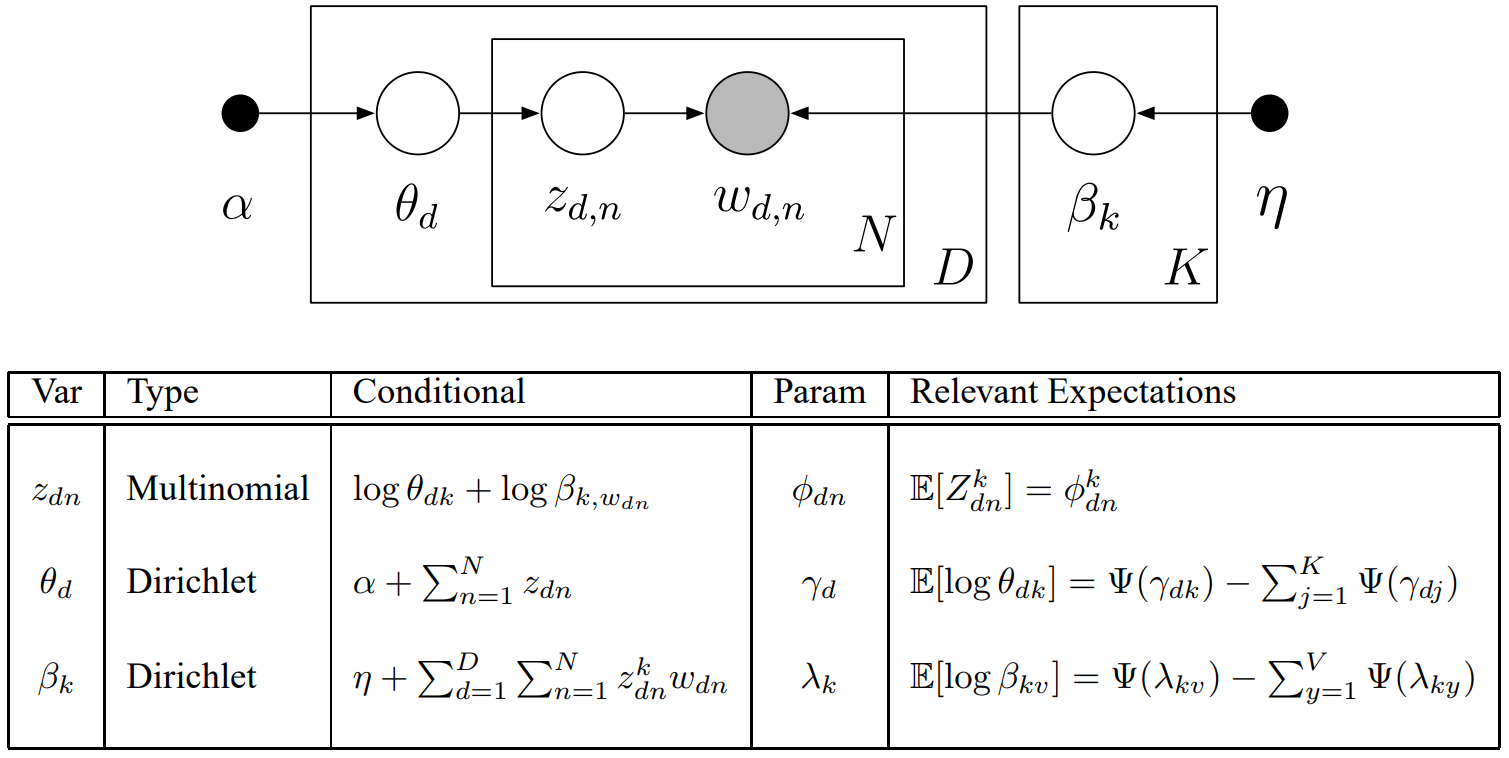
\includegraphics[width=0.95\textwidth]{images/LDA_screenshot.PNG}
    \end{column}
    \begin{column}{0.45\textwidth}
        \footnotesize
        \begin{tabular}{ |c|p{3.8cm}| }
            \hline
            $\alpha$ & Prior of topic\\ & distribution among\\ & documents \\
            \hline
            $\theta_d$ & Distribution of topics\\ & in document $d$ \\
            \hline
            $z_{d,n}$ & Topic for $n^{\text{th}}$ word\\ & in document $d$ \\
            \hline
            $w_{d,n}$ & $n^{\text{th}}$ word in document $d$ \\
            \hline
            $\beta_k$ & Distribution of words in\\ & topic $k$ \\
            \hline
        \end{tabular}
    \end{column}
\end{frame}


\begin{frame}{Generative Process for LDA}
    \begin{itemize}
        \item Draw topics $\beta_k$ $\mathtt{\sim}$ Dirichlet $(\eta,\dots,\eta)$ for $k\in\{1,\dots,K\}$.
        \item For each document $d\in\{1,\dots,D\}$:
        \begin{itemize}
            \item Draw topic proportions $\theta$ $\mathtt{\sim}$ Dirichlet$(\alpha,\dots,\alpha)$
            \item For each word $w\in\{1,\dots,N\}$:
            \begin{itemize}
                \item Draw topic assignment $z_{dn}$ $\mathtt{\sim}$ Multinomial$(\theta_d)$
                \item Draw word $w_{dn}$ $\mathtt{\sim}$ Multinomial($\beta_{z_{dn}}$)
            \end{itemize}
        \end{itemize}
    \end{itemize}
\end{frame}


\begin{frame}{Results from Trial}
    \begin{itemize}
        \item Performing LDA on "Pride and Prejudice" for 10 randomly chosen topics using code from Blei:
        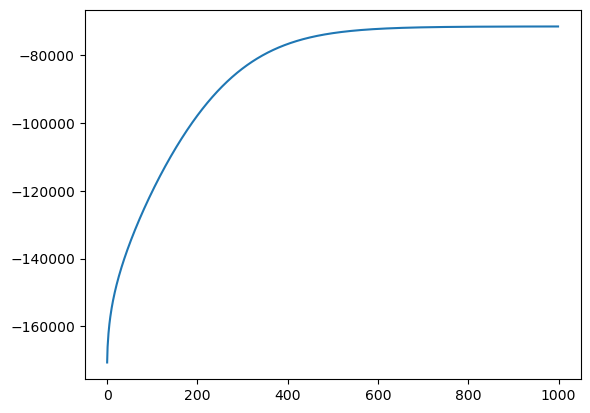
\includegraphics[width=0.4\textwidth]{images/LDA_trial.png}
        \item 20 min for 1000 iterations, vocabulary of 7460 words.
        \begin{itemize}
            \item y-axis represents log predictive probability
            \item x-axis represents number of iterations
        \end{itemize}
    \end{itemize}
\end{frame}



\begin{frame}{Results from Paper}
    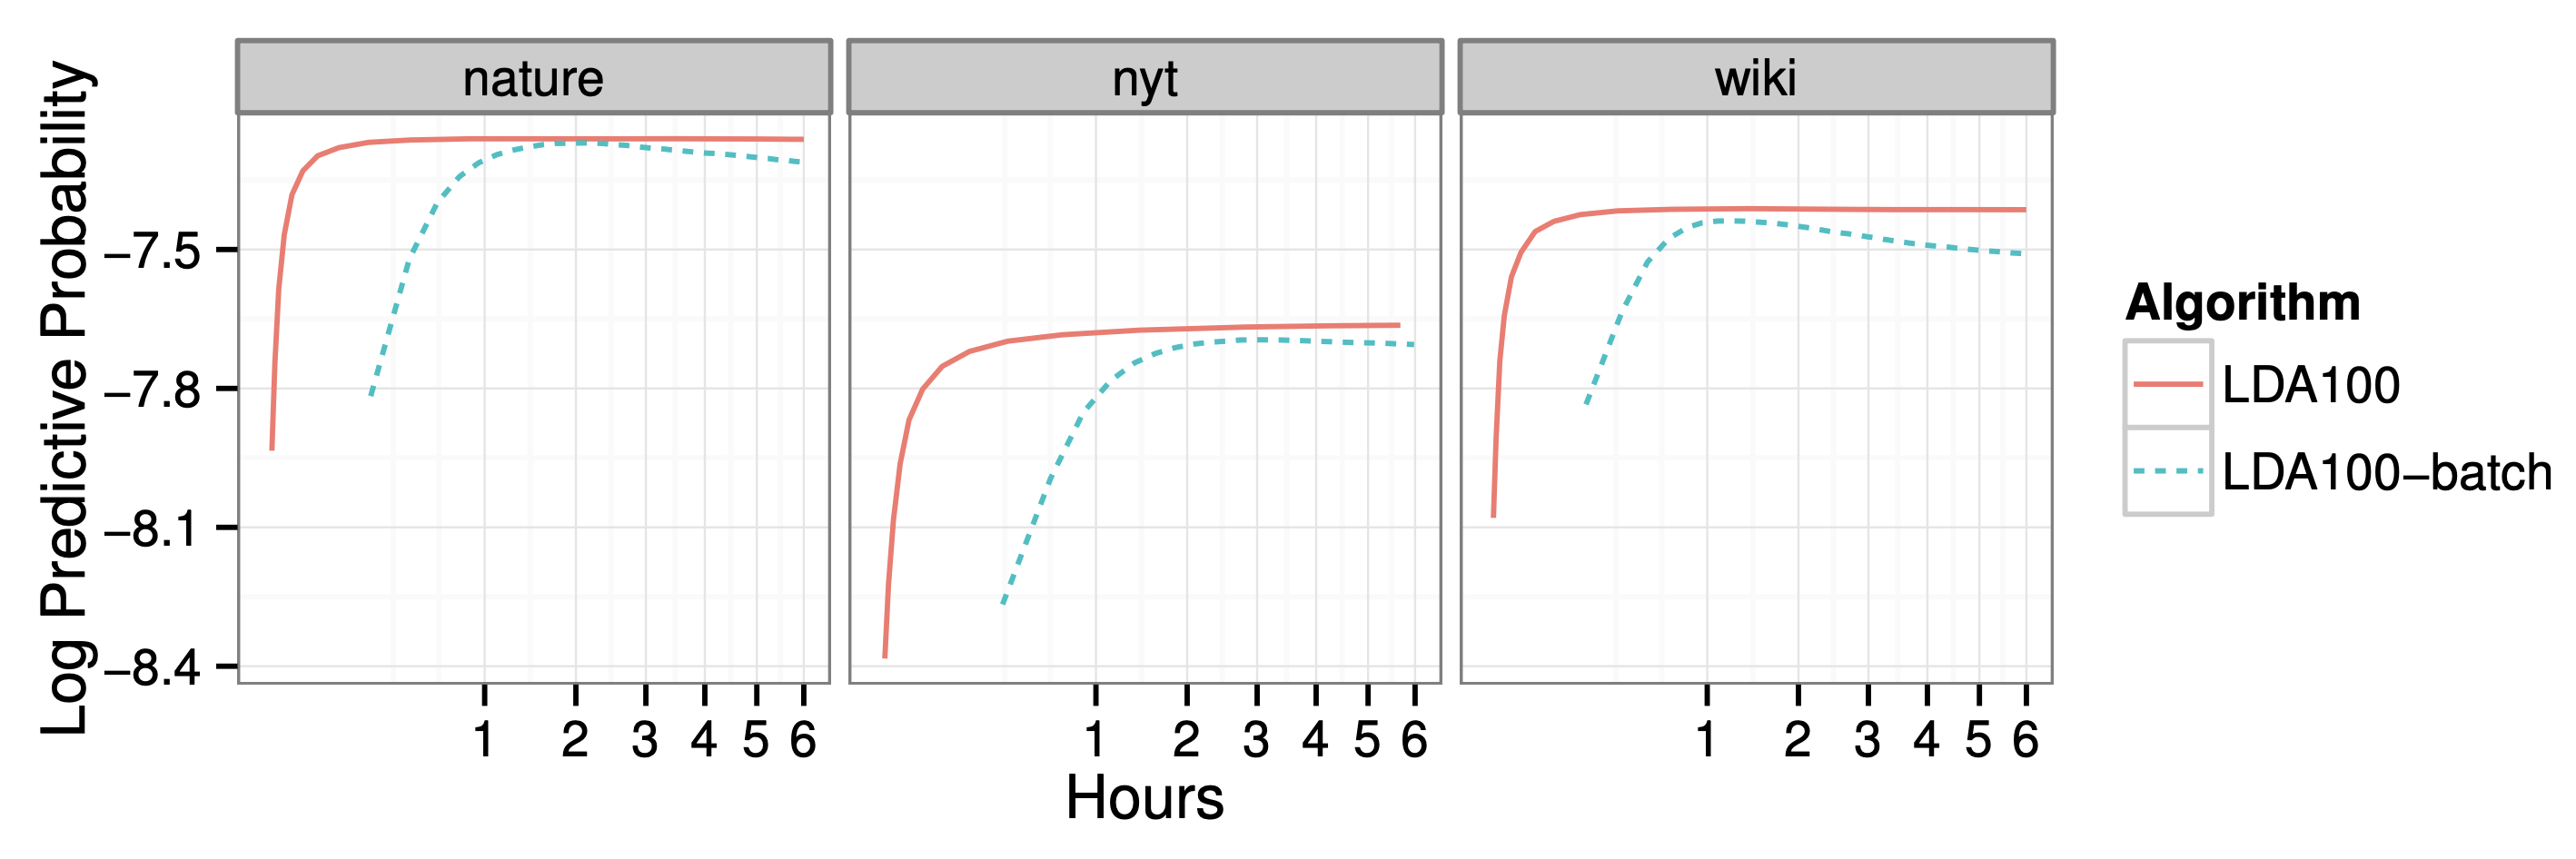
\includegraphics[width=\textwidth]{images/LDA_results_from_paper.png} \\ 
    Pictured: The per-word predictive log likelihood for a 100-topic LDA model on three large corpora. SVI on the full data converges faster and to a better place than batch VI on a reasonably sized subset.
\end{frame}



\begin{frame}[noframenumbering,plain]{Sources}
    \begin{itemize}
        \footnotesize
        \item \url{https://arxiv.org/pdf/1206.7051.pdf}
        \item \url{https://www.cs.princeton.edu/courses/archive/fall11/cos597C/lectures/variational-inference-i.pdf}
        \item \url{https://www.cs.toronto.edu/~madras/presentations/svi-tutorial.pdf}
        \item \url{https://towardsdatascience.com/latent-dirichlet-allocation-lda-9d1cd064ffa2}
        \item \url{https://github.com/lda-project/lda/blob/develop/README.rst}
        \item \url{https://www.kaggle.com/code/pranjalsoni17/topic-modelling-using-lda/notebook#Latent-Dirichlet-Allocation[LDA]:}
        \item \url{https://www.cs.princeton.edu/courses/archive/fall11/cos597C/lectures/variational-inference-i.pdf}
        \item
        \url{https://arxiv.org/pdf/1601.00670.pdf}
    \end{itemize}
\end{frame}



\begin{frame}[noframenumbering,plain]
    \begin{center}
        \Huge \textcolor{end_title_color}{Thank You!}
    \end{center}
\end{frame}



\end{document}

% =============================================================
% =========================== END =============================
% =============================================================
